\documentclass[a4paper,10pt]{article}
\usepackage[utf8]{inputenc}
\usepackage{polski}
\usepackage{graphicx}

\title{Specyfikacja wymagań}
\author{Magdalena Grabowska, Daniel Oklesiński, Wojciech Opydo}

\begin{document}

\maketitle
\section{Wprowadzenie}
Tworzona aplikacja służy do nauki słów z języków obcych. W bazie danych przechowywane są zbiory słów z języka obcego wraz z ich tłumaczeniami na język polski (zbiory te będą dalej nazywane słownikami). Każdy słownik ma przypisaną kategorię słów do których się odnosi (np. żywność, sport, szkoła), język (np. angielski, niemiecki, hiszpański) oraz poziom trudności. Na podstawie słownika tworzony jest quiz mający na celu sprawdzenie znajomości jego słówek. Pytania quizu polegają na tłumaczeniu słów z języka polskiego na język słownika lub odwrotnie. Możliwe są różne rodzaje pytań, między innymi: zamknięte (mając dane słowo, wybierz, która z podanych kilku odpowiedzi jest poprawnym tłumaczeniem) i otwarte (wpisz z klawiatury tłumaczenie danego słowa).
\section{Wymagania}
\subsection{Funkcjonalne}
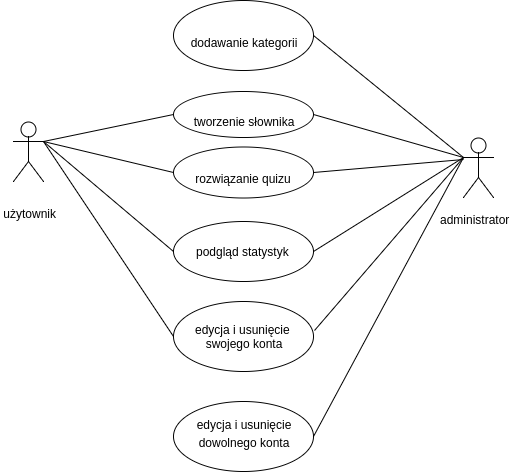
\includegraphics[scale=0.55]{use_cases}
%\begin{enumerate}
%\item Użytkownik może założyć i usunąć swoje konto.
%\item Administrator może tworzyć i usuwać dowolne konta.
%\item Użytkownik może tworzyć dodać słownik, wypełnić quiz stworzony na jego podstawie, lub na podstawie słownika dodanego przez innego użytkownika
%\item Użytkownik może usuwać stworzone przez siebie słowniki.
%\item Administrator może usuwać wszystkie słowniki.
%\item Użytkownik może oglądać swoje statystyki oraz statystyki innych użytkowników
%\item Możliwość wyszukiwania słowników przez kategorię, język i trudność. 
%\item Możliwość wyboru rodzaju pytań w wygenerowanym quzie.
%\end{enumerate}
%\subsubsection{Przypadki użycia}
%\begin{enumerate}
%\item Uczeń chcący nauczyć się pewnej liczby słówek na lekcję angielskiego, tworzy nowy słownik zawierający te słówka, a następnie generowany jest quiz, który wypełnia. Może wysłać link do słownika kolegom z klasy, którzy uczą się tych samych słówek.
%\item Osoba jadąca na wycieczkę do Hiszpanii chciałaby się nauczyć podstawowych zwrotów w tym języku. W tym celu może wyszukać słownik o najniższym poziomie, języku hiszpańskim i odpowiedniej kategorii. Jeśli taki słownik został już stworzony przez jakiegoś użytkownika, może ona zacząć naukę.
%\end{enumerate}
\subsection{Pozafunkcjonalne}
\begin{enumerate}
\item Strona jest responsywna. Działa poprawnie na urządzeniach mobilnych.
\item Strona działa poprawnie na przeklądarkach: Google Chrome, Mozilla Firefox, Safari, Opera.
\item Korzystanie z aplikacji nie wymaga zakupu jakiegokolwiek oprogramowania.
\item Ze strony może korzystać jednocześnie 100 użytkowników.
\item Strona nie powinna posiadać ograniczenia na liczbę użytkowników ani liczbę słowników. 
\end{enumerate}
\end{document}
